% ----------------------------------------
% ----------------------------------------
% Report template
% Author: Miloš D. Petrašinović <mpetrasinovic@mas.bg.ac.rs>
% Faculty of Mechanical Engineering, University of Belgrade
% Department of Aerospace Engineering, Flying structures
% https://vazmfb.com
% Belgrade, 2023
% ----------------------------------------
% ----------------------------------------

% ----------------------------------------
% Used packages definition and document format
% ----------------------------------------
\documentclass[12pt,oneside]{book}
\usepackage{geometry}
\usepackage[cmyk]{xcolor}
\usepackage{listings}
\usepackage[numbered]{matlab-prettifier}
\usepackage[T1]{fontenc}
\usepackage[utf8]{inputenc}
\usepackage{lmodern}
\usepackage[unicode]{hyperref}
\usepackage{graphicx}
\usepackage[english]{babel}
\usepackage{csquotes}
\usepackage[style=ieee]{biblatex}
\usepackage{emptypage}
\usepackage{textcomp}
\usepackage{placeins}
\usepackage{amssymb}
\usepackage{amsmath}
\usepackage[toc,title]{appendix}
\usepackage{nomencl}
\usepackage{fancyhdr}
\usepackage{titlesec}
\usepackage{indentfirst}
\usepackage{float}
\usepackage{caption}
\usepackage{bigstrut}
\usepackage{booktabs}
\usepackage{colortbl}
\usepackage{multirow}
\usepackage{enumitem}
\usepackage{tocbasic}
\usepackage{siunitx}
\usepackage{array}
\usepackage{fancyvrb}
\usepackage{icomma}
\usepackage{bm}
\usepackage{tikz}
\usepackage{scalerel}

% Literature
\addbibresource{bibliography.bib}

% Folder for figures
\graphicspath{{figures/}}

% Colors
\definecolor{tamno-plava}{cmyk}{1,0.79,0.32,0.17}
\definecolor{svetlo-plava}{cmyk}{0.93,0.64,0.03,0}
\definecolor{siva}{cmyk}{0.73,0.67,0.65,0.8}
\definecolor{tamno-siva}{HTML}{aaaaaa}
\definecolor{zelena}{cmyk}{1,0,1,0.5}

% Comma-separated numbers
%\mathcode`\.=\numexpr\mathcode`\,-"6000\relax

% Matrix 
\makeatletter
\renewcommand*\env@matrix[1][c]{\hskip -\arraycolsep
  \let\@ifnextchar\new@ifnextchar
  \array{*\c@MaxMatrixCols #1}}
\makeatother

% Norms
\newcommand{\norm}[1]{\left\lVert#1\right\rVert}
\newcommand{\abs}[1]{\left\lvert#1\right\rvert}
\newcommand{\diff}[1]{\mathrm{d}#1}

% Matlab code
\lstset{
  style = Matlab-editor,
  basicstyle = \fontfamily{pcr}\selectfont\footnotesize, % if you want to use Courier
  numberstyle = \tiny\color{siva},
  commentstyle = \color{zelena},
}

% Units of measurement
\sisetup{
  per-mode=fraction,
  fraction-function=\tfrac
}

% Spacing management
\captionsetup[figure]{belowskip=-12pt}
\setlength{\jot}{6pt}
\raggedbottom
\DeclareTOCStyleEntry[dynnumwidth]{tocline}{section}
\DeclareTOCStyleEntry[dynnumwidth]{tocline}{figure}
\DeclareTOCStyleEntry[dynnumwidth]{tocline}{table}

% Brackets in formulas
\delimitershortfall=-1pt

% No continuation in the next row
\tolerance=1
\emergencystretch=\maxdimen
\hyphenpenalty=10000
\hbadness=10000

% Paper size
\geometry{
  paperheight=297mm,
  paperwidth=210mm,
  top=20mm,
  bottom=20mm,
  right=20mm,
  left=25mm,
  headheight=16pt
}

% Index and nomenclature
\usepackage{makeidx}
\makeindex 
\usepackage[totoc]{idxlayout} 
\makenomenclature
 
% ORCID
\usetikzlibrary{calc}
\usetikzlibrary{shadings} 
\usetikzlibrary{svg.path}
\definecolor{orcidlogocol}{HTML}{A6CE39}
\tikzset{
  orcidlogo/.pic={
    \fill[orcidlogocol] svg{M256,128c0,70.7-57.3,128-128,128C57.3,256,0,198.7,0,128C0,57.3,57.3,0,128,0C198.7,0,256,57.3,256,128z};
    \fill[white] svg{M86.3,186.2H70.9V79.1h15.4v48.4V186.2z}
                 svg{M108.9,79.1h41.6c39.6,0,57,28.3,57,53.6c0,27.5-21.5,53.6-56.8,53.6h-41.8V79.1z M124.3,172.4h24.5c34.9,0,42.9-26.5,42.9-39.7c0-21.5-13.7-39.7-43.7-39.7h-23.7V172.4z}
                 svg{M88.7,56.8c0,5.5-4.5,10.1-10.1,10.1c-5.6,0-10.1-4.6-10.1-10.1c0-5.6,4.5-10.1,10.1-10.1C84.2,46.7,88.7,51.3,88.7,56.8z};
  }
}

\newcommand\orcid[2]{\href{https://orcid.org/#2}{#1 \mbox{\scalerel*{

\begin{tikzpicture}[yscale=-1,transform shape]
\pic{orcidlogo};
\end{tikzpicture}
}{|}}}}

% Title style
\titleformat{\chapter}[display]
{\normalfont\Huge\bfseries\raggedright}{ 
    \fcolorbox{siva}{siva}{\textcolor{white}{
        \raisebox{10pt}[35pt][0pt]{ \thechapter }
    }}}
  {10pt}{\Huge}[\titleline{\color{siva}\vspace{10pt}\titlerule}]

\makeatletter
\renewcommand\@seccntformat[1]{%
  \textcolor{siva}{\csname the#1\endcsname}
}
\makeatother

% Header style
\fancypagestyle{tekst}{
    \setlength{\parskip}{6pt}
    \fancyhf{}
    \fancyhead[RO]{\bfseries\slshape \color{black}\leftmark}
    \fancyhead[LO]{\bfseries}
    \cfoot{\bfseries \color{black}\thepage}
    \renewcommand{\headrulewidth}{0.4pt}
    \renewcommand{\headrule}{\color{siva}\hrule}
    \renewcommand{\footrulewidth}{0.4pt}
    \renewcommand{\footrule}{\color{siva}\hrule}

}

\fancypagestyle{sazetak}{
    \setlength{\parskip}{1pt}
    \fancyhf{}
    \fancyhead[RO]{\bfseries\slshape \leftmark}
    \fancyhead[LO]{\bfseries}
    \cfoot{\bfseries \color{black}\thepage}
    \renewcommand{\headrulewidth}{0.4pt}
    \renewcommand{\headrule}{\color{siva}\hrule}
    \renewcommand{\footrulewidth}{0.4pt}
    \renewcommand{\footrule}{\color{siva}\hrule}
}

\fancypagestyle{listing}{
    \setlength{\parskip}{1pt}
    \fancyhf{}
    \fancyhead[RO]{\bfseries\slshape \leftmark}
    \fancyhead[LO]{\bfseries}
    \cfoot{\bfseries \color{black}\thepage}
    \renewcommand{\headrulewidth}{0.4pt}
    \renewcommand{\headrule}{\color{siva}\hrule}
    \renewcommand{\footrulewidth}{0.4pt}
    \renewcommand{\footrule}{\color{siva}\hrule}
}

\fancypagestyle{plain}{
  \fancyhf{}%
  \cfoot{\bfseries \color{black}\thepage}
  \renewcommand{\footrulewidth}{0.4pt}
  \renewcommand{\headrulewidth}{0pt}
  \renewcommand{\headrule}{}
}

% Figures caption settings
\DeclareCaptionLabelSeparator{bar}{ - }
\captionsetup{labelsep=bar}

% ----------------------------------------
% Defining the chapter - DEDICATION
% ----------------------------------------
\newenvironment{dedication}
{
   \cleardoublepage
   \thispagestyle{empty}
   \vspace*{\stretch{1}}
   \hfill\begin{minipage}[t]{0.66\textwidth}
   \raggedleft
}
{
   \end{minipage}
   \vspace*{\stretch{3}}
   \clearpage
}

% ----------------------------------------
% Defining an element - QUOTE
% ----------------------------------------
\makeatletter
\renewcommand{\@chapapp}{}
\newenvironment{chapquote}[2][2em]
  {\setlength{\@tempdima}{#1}%
   \def\chapquote@author{#2}%
   \parshape 1 \@tempdima \dimexpr\textwidth-2\@tempdima\relax%
   \itshape}
  {\par\normalfont\hfill--\ \chapquote@author\hspace*{\@tempdima}\par\bigskip}
\makeatother

% ----------------------------------------
% BEGINNING OF THE DOCUMENT
% ----------------------------------------
\begin{document}

% ----------------------------------------
% NASLOVNA STRANA
% ----------------------------------------
\frontmatter
\begin{titlepage}
	\centering
	\vspace*{\fill}
	
    \href{http://vaz.mas.bg.ac.rs/}{
\includegraphics[height=2.5cm]{vaz-logo-t}}
    \hspace{0.2cm}
    \href{https://www.mas.bg.ac.rs/}{
\includegraphics[height=2.5cm]{mfb-logo-t}}
    \hspace{0.2cm}
    \href{https://www.bg.ac.rs/}{
\includegraphics[height=2.5cm]{ub-logo-t}}
    
    \vspace{0.5cm}
    
    {\scshape \LARGE \href{https://www.bg.ac.rs/}{\textcolor{tamno-siva}{University of Belgrade}}\par \href{https://www.mas.bg.ac.rs/}{Faculty of Mechanical Engineering}\par \href{http://vaz.mas.bg.ac.rs/}{\textcolor{tamno-plava}{Aerospace Engineering Department}}\par} % Na engleskom 
    %{\scshape \LARGE \href{https://www.bg.ac.rs/}{\textcolor{tamno-siva}{Univerzitet u Beogradu}}\par \href{https://www.mas.bg.ac.rs/}{Mašinski fakultet}\par \href{http://vaz.mas.bg.ac.rs/}{\textcolor{tamno-plava}{Katedra za vazduhoplovstvo}}\par} % Na srpskom 
    \vspace{0.5cm}
    %

\noindent\hspace{-0.5cm}\makebox[\linewidth]{\textcolor{svetlo-plava}{\rule{\paperwidth}{5pt}}}
	
	\vspace{5cm}
	{\Large \itshape Course title \par} % Enter course title
	\vspace{0.5cm}
	{\color{siva}\Huge \textbf{Report title} \par} % Enter the title and date
	\vspace{0.5cm}
	{\Large \itshape \orcid{First name Last Name}{0000-0000-0000-0000}\par} % Replace first and last name and 0000-0000-0000-0000 with ORCID
	\vspace{5mm}
	{\large \href{https://vazmfb.com/course/}{\texttt{vazmfb.com/course/}}} % Enter address
	\vspace*{\fill}
	\vfill

	{\large \textsc{Belgrade, 2023}} % Place and year
\end{titlepage}

% ----------------------------------------
% THE CONTENT
% ----------------------------------------
\pagestyle{listing}
\cleardoublepage
\phantomsection
\addcontentsline{toc}{chapter}{\contentsname}
\tableofcontents

% ----------------------------------------
% FIGURES LISTING AND LISTING TABLE
% ----------------------------------------
\pagestyle{listing}
\cleardoublepage
\phantomsection
\addcontentsline{toc}{chapter}{\listfigurename}
\listoffigures
\cleardoublepage
\phantomsection
\addcontentsline{toc}{chapter}{\listtablename} 
\listoftables

% ----------------------------------------
% LISTING OF MARKS AND ABBREVIATIONS
% ----------------------------------------
\cleardoublepage
\phantomsection
\markboth{\MakeUppercase \nomname}{\MakeUppercase \nomname}
\addcontentsline{toc}{chapter}{\nomname}
\printnomenclature

% ----------------------------------------
% PROGRAM LISTING
% ----------------------------------------
\cleardoublepage
\phantomsection
\addcontentsline{toc}{chapter}{\lstlistlistingname}
\lstlistoflistings

% ----------------------------------------
% BEGINNING OF THE TEXT
% ----------------------------------------
\mainmatter
\pagestyle{tekst}

% ----------------------------------------
% CHAPTER
% ----------------------------------------
\chapter{Chapter One}

\begin{chapquote}{\textit{First name Last Name}\index{First name Last Name}\footnote{Footnote text about this author}}
``Something very smart and related to the topic...''
\end{chapquote}

First chapter text 

% ----------------------------------------
% SECTION
% ----------------------------------------
\section{First section}

Inserting an image (image \ref{orao}) into the report % Referencing with \label and \ref

\begin{figure}[H]
    \centering
    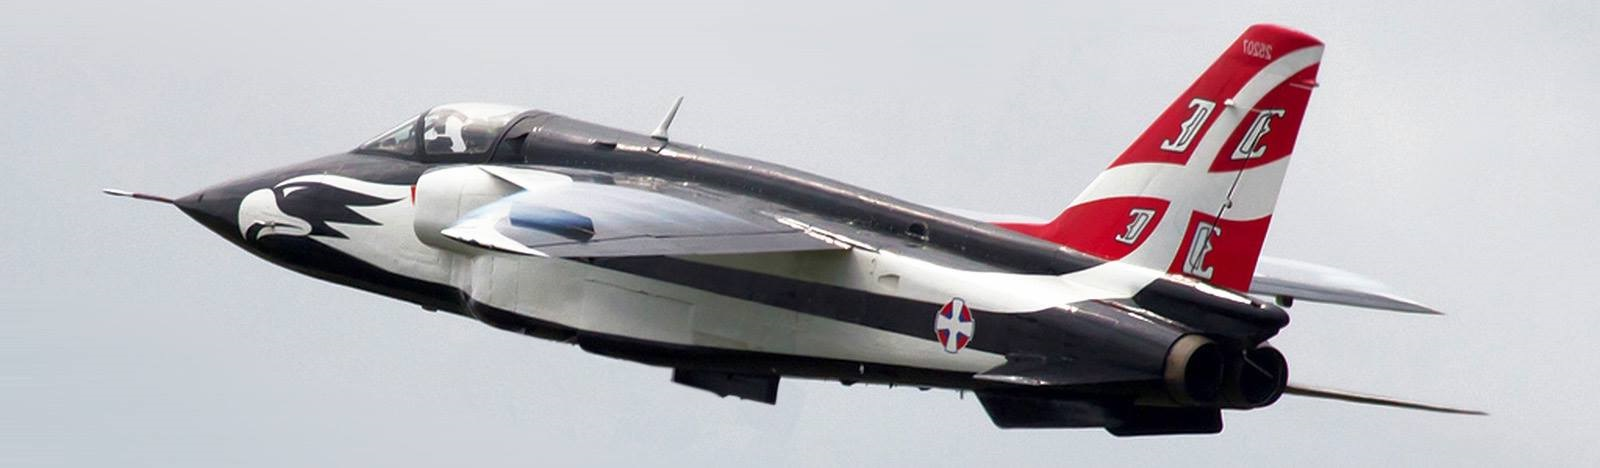
\includegraphics[width=0.9\textwidth]{orao}
    \caption{Figure caption}
    \label{orao}
\end{figure}

% ----------------------------------------
% SUBSECTON
% ----------------------------------------
\subsection{First subsection}

Lists and two columns on page

\vspace{1cm} % vertical distance

% Left half
\begin{minipage}{0.4\textwidth}
    \begin{itemize}
    	\item First 
    	\item Second
    	\item Third
    \end{itemize}
\end{minipage}
% Right half
\begin{minipage}{0.4\textwidth}
    \begin{enumerate}
    	\item First 
    	\item Second
    	\item Third
    \end{enumerate}
\end{minipage}

% ----------------------------------------
% CHAPTER
% ----------------------------------------
\chapter{New chapter}

\textit{Website address with link:} % Italic text
\url{https://vazmfb.com}

\href{https://vazmfb.com}{Text with link to vazmfb.com}

Equation \ref{eq1} % The equation and all other elements are referenced in the same way
\begin{equation}
    \label{eq1}
    \Pi = \frac{1}{2} \int_{V} \bm{\varepsilon}^T\, \bm{\sigma}\, \text{d}V = \frac{1}{2} \int_{V} \bm{\varepsilon}^T\, \bm{c}\, \bm{\varepsilon}\, \diff{V}
    \nomenclature{$\Pi$}{Potential energy}
    \nomenclature{$V$}{Body volume}
    \nomenclature{$\bm{\sigma}$}{Stress tensor}
    \nomenclature{$\bm{\varepsilon}$}{Deformation vector}
    \nomenclature{$\bm{c}$}{Matrix of elastic characteristics of materials}
\end{equation}

Program example:
\lstinputlisting[language=Matlab, caption=Program caption]{programs/program.m}

Example of \textbf{matrix equations} % Bold text
\footnotesize
\begin{equation}
    \begin{bmatrix}
       \sigma_{xx} \\
       \sigma_{yy} \\
       \sigma_{zz} \\
       \sigma_{yz} \\
       \sigma_{xz} \\
       \sigma_{xy} \\
    \end{bmatrix} 
     = 
    \begin{bmatrix}
       c_{11} & c_{12} & c_{13} & c_{14} & c_{15} & c_{16} \\
       & c_{22} & c_{23} & c_{24} & c_{25} & c_{26} \\
       & & c_{33} & c_{34} & c_{35} & c_{36} \\
       & & & c_{44} & c_{45} & c_{46} \\
       & & & & c_{55} & c_{56} \\
       \multicolumn{2}{c}{\text{Sim.}} & & & & c_{66} \\
    \end{bmatrix} 
    \begin{bmatrix}
       \varepsilon_{xx} \\
       \varepsilon_{yy} \\
       \varepsilon_{zz} \\
       \gamma_{yz} \\
       \gamma_{xz} \\
       \gamma_{xy} \\
    \end{bmatrix} 
\end{equation}

Example of literature citation\cite{petrasinovic22}.
 
% ----------------------------------------
% LITERATURA
% ----------------------------------------
\pagestyle{listing}
\hyphenpenalty=1
\hbadness=1

\cleardoublepage
\phantomsection
\addcontentsline{toc}{chapter}{\bibname} 
\printbibliography

% ----------------------------------------
% APPENDIX
% ----------------------------------------
\begin{appendices}

% ----------------------------------------
% CHAPTER
% ----------------------------------------
\chapter{Some appendix}
Appendix text

Example table

\begin{table}[H]
\large
\centering
\caption{Table caption}
\begin{tabular}[H]{|l|c|}
\hline
First cell & Right \\ \hline
Down & Diagonal \\ \hline
\end{tabular}
\end{table}

\end{appendices}

% ----------------------------------------
% INDEKS
% ----------------------------------------
% It is written with the text \index{text}
\printindex 

% ----------------------------------------
% END OF DOCUMENT
% ----------------------------------------
\end{document}